%! Author = Robert Kulesa, Daniel Liu, Michael Li
%! Date = 11/4/2021

% Preamble
\documentclass[11pt]{article}

% Packages
\usepackage{amsmath}
\usepackage{graphicx}

% Document
\begin{document}
    \begin{titlepage}
        \begin{center}
            \vspace{1cm}

            \Huge
            \textbf{Adversarial Search * Bayesian Networks}

            \vspace{0.5cm}
            \LARGE
            Assignment 3

            \vspace{1cm}

            \textbf{Michael Li - 192008938}

            \textbf{Daniel Liu - 184007283}

            \textbf{Robert Kulesa - 185009892}


            \vfill


            \vspace{0.8cm}

            \Large
            CS440 Fall 2021\\
            Professor Boularias\\
            Rutgers University - New Brunswick\\
            November 30, 2021

        \end{center}
    \end{titlepage}

    \begin{center}
        \Large
        \textbf{Problem 1}
    \end{center}
    \normalsize
    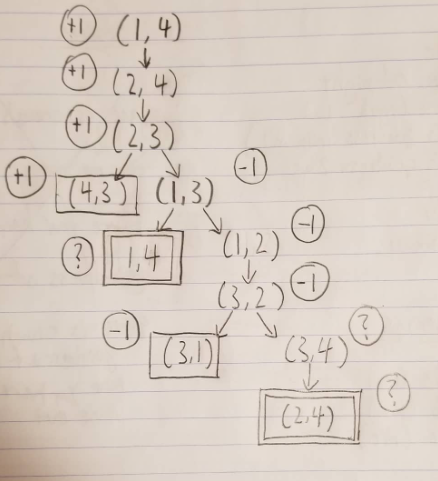
\includegraphics[width=\linewidth]{images/game_tree} \\
    "?" values are used to annotate loop states. When an agent has to choose between a +1 value and a "?" value (+1,?) the max player will always choose +1 while the min player will choose ?, and vice versa for (-1,?), with the min player choosing -1 and the max player choosing "?". Since the game value of a loop state is unknown, it is best for a max/min player to choose the corresponding max/min value if it is available, however if that value is not available the "?" state is a viable option to explore as it cannot be worse than an immediate loss. If all the successors of a state have a "?" value, the backed-up value is also "?".

    \begin{center}
        \Large
        \textbf{Problem 2}
    \end{center}
    \normalsize
    \begin{enumerate}

        
    \end{enumerate}

    \begin{center}
        \Large
        \textbf{Problem 3}
    \end{center}
    \normalsize

    \begin{center}
        \Large
        \textbf{Problem 4}
    \end{center}
    \normalsize


    


\end{document}
